\begin{subfigure}[c][][l]{0.45\textwidth}
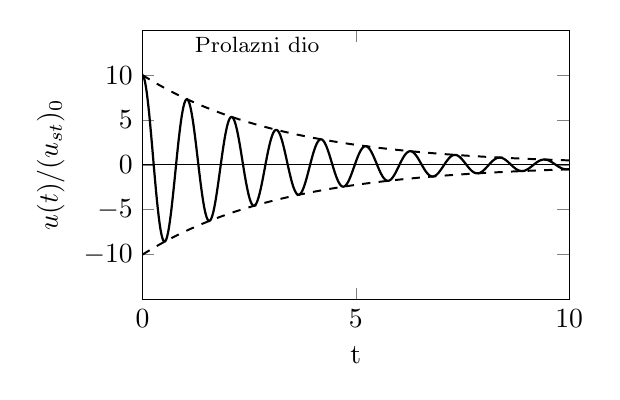
\begin{tikzpicture}
\begin{axis} [
    title={\footnotesize{Prolazni dio}},
    title style={at={(0.1,0.95)}, anchor=north west, draw=none, fill=none},
    height=5cm,
    width=7cm,
    xlabel=t,ylabel=$u(t)/(u_{st})_0$,
    ylabel near ticks, ylabel style={anchor=south},
    xmin = 0, xmax = 10,
    ymin = -15, ymax = 15,
    xtick = {0, 5, 10, 15, 20},
    ytick = {-10, -5, 0, 5, 10},
 ]
    \draw[thin] (0,0) -- (20,0);
    \addplot [
        domain=0:20,
        samples=200,
        color=black,
        dashed,line width=0.25mm,
    ] {10*exp(-0.05*6*x)};
    \addplot [
        domain=0:20,
        samples=200,
        color=black,
        dashed,line width=0.25mm,
    ] {-10*exp(-0.05*6*x)};
    \addplot [
        domain=0:20,
        samples=1000,
        color=black,
        thick,
    ] {10*exp(-0.05*6*x)*cos(6*deg(x))};
\end{axis}
\end{tikzpicture}
\end{subfigure}
\hfill
%
%
%
\begin{subfigure}[b][][r]{0.05\textwidth}
    \centering
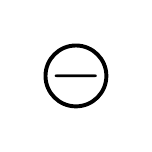
\begin{tikzpicture}[scale=5]
    \draw[thick, line width=0.5mm] (0,0) circle (2.2pt);
    \node[circle,fill=none,color=black] at (0,0) {\textbf{\Huge{$-$}}};
\end{tikzpicture}
\end{subfigure}
\hfill
%
%
%
\begin{subfigure}[c][][r]{0.45\textwidth}
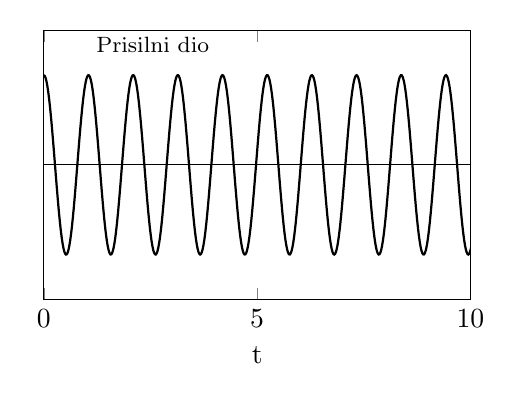
\begin{tikzpicture}
\begin{axis} [
    title={\footnotesize{Prisilni dio}},
    title style={at={(0.1,0.95)}, anchor=north west, draw=none, fill=none},
    height=5cm,
    width=7cm,
    xlabel=t,%ylabel=$u(t)/(u_{st})_0$,
%    ylabel near ticks, ylabel style={anchor=south},
    xmin = 0, xmax = 10,
    ymin = -15, ymax = 15,
    xtick = {0, 5, 10, 15, 20},
%    ytick = {-10, -5, 0, 5, 10},
    ytick=\empty,
 ]
    \draw[thin] (0,0) -- (20,0);
    \addplot [
        domain=0:20,
        samples=1000,
        color=black,
        thick,
    ] {10*cos(6*deg(x))};
\end{axis}
\end{tikzpicture}
\end{subfigure}
\vfill
%
%
%
\begin{subfigure}[b][3pt][c]{1\textwidth}
    \centering
    
\begin{tikzpicture}[scale=5]
        \draw[thick, line width=0.5mm] (0,0) circle (2.2pt); 
        \node[circle,fill=none,color=black] at (0,0) {\textbf{\Huge{$=$}}};
    \end{tikzpicture}
\end{subfigure}
\vfill
%
%
%
\begin{subfigure}[t][][c]{1\textwidth}
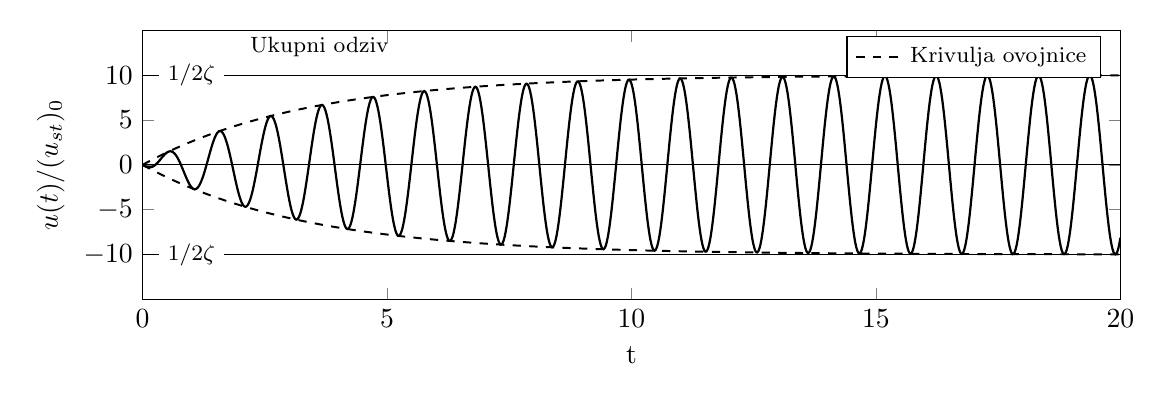
\begin{tikzpicture}
\begin{axis} [
    title={\footnotesize{Ukupni odziv}},
    title style={at={(0.1,0.95)}, anchor=north west, draw=none, fill=none},
    height=5cm,
    width=14cm,
    xlabel=t,ylabel=$u(t)/(u_{st})_0$,
    ylabel near ticks, ylabel style={anchor=south},
    xmin = 0, xmax = 20,
    ymin = -15, ymax = 15,
    xtick = {0, 5, 10, 15, 20},
    ytick = {-10, -5, 0, 5, 10},
 ]
    \draw[thin] (0,0) -- (20,0);

    \addplot [
        domain=0:20,
        samples=200,
        color=black,
        dashed,line width=0.25mm,
    ] {10*(exp(-0.05*6*x)-1)};

    \addplot [
        domain=0:20,
        samples=200,
        color=black,
        dashed,line width=0.25mm,
    ] {-10*(exp(-0.05*6*x)-1)};

    \addlegendentry{\footnotesize{Krivulja ovojnice}}

    \addplot [
        domain=0:20,
        samples=1000,
        color=black,
        thick,
    ] {10*exp(-0.05*6*x)*cos(6*deg(x))-10*cos(6*deg(x))};
%    \addlegendentry{\footnotesize{Ukupni odziv}}


    
    \draw[thin] (0,10) -- (20,10);
    \node[rectangle, fill=white] at (1,10) {\footnotesize{$1/2\zeta$}};
    \draw[thin] (0,-10) -- (20, -10);
    \node[rectangle, fill=white] at (1,-10) {\footnotesize{$1/2\zeta$}};

    \end{axis}
\end{tikzpicture}
\end{subfigure}

